\begin{figure}
\centering
\begin{tikzpicture}
  \node {
    \begin{tikzpicture}
      \node[inner sep=0pt] (circuit) at (0,0) {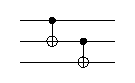
\includegraphics[scale=2]{Figures/circuits/interchangeCNOTs1}};
      \node[right=0mm of circuit.north west, font=\itshape] (text) {a)};
      \node[above right=0.8mm and 13.1mm of circuit.west, opacity=0.9] {\footnotesize \(\alpha\)};
      \node[below right=0.8mm and 23.7mm of circuit.west, opacity=0.9] {\footnotesize \(\beta\)};
    \end{tikzpicture}
    \hspace{8mm}
    \begin{tikzpicture}
      \node[inner sep=0pt] (circuit) at (0,0) {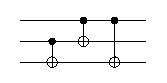
\includegraphics[scale=2]{Figures/circuits/interchangeCNOTs2}};
      \node[right=0mm of circuit.north west, font=\itshape] (text) {b)};
      \node[above right=0.8mm and 23.7mm of circuit.west, opacity=0.9] {\footnotesize \(\alpha\)};
      \node[below right=0.8mm and 13.1mm of circuit.west, opacity=0.9] {\footnotesize \(\beta\)};

    \end{tikzpicture}
  };
\end{tikzpicture}
\caption{Equivalent circuits with the two gates in \textit{a)} being interchanged in \textit{b)}. A byproduct CNOT gate is created in the process.}
\label{fig:interchangeRule}
\end{figure}